% SSU Data Dash 2026 report (solo submission) -- draft v2, written from the R script.
% Put this file in report/ of the repository. It reads files that the R script creates:
%   ../reports/numbers.tex, ../reports/results_table.tex, ../reports/error_by_type.tex
%   ../figures/error_by_price_range.png, ../figures/importance.png
% Compile on Overleaf (upload the whole repository as a zip) or: pdflatex report.tex (twice).
% Keep the report to 4 pages, not counting the outside-data table and the appendix.
\documentclass[11pt]{article}
\usepackage[margin=2.2cm]{geometry}
\usepackage{graphicx,booktabs,hyperref,xcolor,amsmath}
\graphicspath{{../figures/}}
\setlength{\parskip}{4pt}
\newcommand{\todo}[1]{\textcolor{red}{\textbf{[TODO: #1]}}}
\newcommand{\nTrain}{150{,}000}
\newcommand{\nValOff}{10{,}069}
\newcommand{\nValLa}{10{,}069}
\newcommand{\nTestOff}{3{,}974}
\newcommand{\nTestLa}{4{,}064}
\newcommand{\gapMonths}{2}
\newcommand{\offMdAPE}{11.4}
\newcommand{\offMAPE}{14.5}
\newcommand{\offBaseMdAPE}{18.0}
\newcommand{\offOlsMdAPE}{17.2}
\newcommand{\offGainBase}{36}
\newcommand{\offGainOls}{34}
\newcommand{\laMdAPE}{5.7}
\newcommand{\laMAPE}{6.7}
\newcommand{\laBaseMdAPE}{7.3}
\newcommand{\laGainBase}{21}
\newcommand{\offBiasPct}{-0.4}
\newcommand{\laBiasPct}{+4.2}
\newcommand{\worstType}{Co-Op Apt}
\newcommand{\worstTypeMd}{14.7}
\newcommand{\bestType}{Condo Townhouse}
\newcommand{\bestTypeMd}{8.9}
\newcommand{\worstDecile}{10}
\newcommand{\worstDecileMd}{21.3}
\newcommand{\bestDecile}{3}
\newcommand{\bestDecileMd}{7.8}
\newcommand{\worstDecilePriceLo}{1{,}763{,}000}
\newcommand{\laWorstDecile}{1}
\newcommand{\laWorstDecileMd}{7.9}
\newcommand{\worstMonth}{2025-12}
\newcommand{\worstMonthMd}{12.7}
\newcommand{\bestMonth}{2026-03}
\newcommand{\bestMonthMd}{10.9}
\newcommand{\worstMuni}{Scarborough}
\newcommand{\worstMuniMd}{12.0}
\newcommand{\offTopA}{ols\_fund}
\newcommand{\offTopB}{community}
\newcommand{\offTopC}{area\_mid}
\newcommand{\laTopA}{list\_vs\_ols}
\newcommand{\laTopB}{log\_list}
\newcommand{\laTopC}{community}
\newcommand{\indexLevel}{-0.025}
\newcommand{\trendUsed}{held flat at the average of its last three months for the off-market model and extrapolated linearly for the list-aware model}


\title{SSU Data Dash 2026: A de-trended random forest for Toronto-area home prices}
\author{\todo{your full name}}
\date{}

\begin{document}
\maketitle

\noindent\begin{tabular}{@{}ll}
\textbf{Video (YouTube, unlisted is fine):} & \url{https://youtu.be/YOUR-VIDEO} \\
\textbf{Code and submission files (GitHub):} & \url{https://github.com/erwinzhang7/SSU-Data-Dash} \\
\end{tabular}

\section*{Summary}
We predict sold prices with random forests fitted to log prices, after removing a market-wide price trend estimated from past sales only. Tested walk-forward on later months (Dec 2025--May 2026), the off-market model reaches a median absolute percentage error (MdAPE) of \offMdAPE\% against \offBaseMdAPE\% for a group-median baseline, and the list-aware model reaches \laMdAPE\% against \laBaseMdAPE\% for simply using the list price. The main finding is that most of the gain comes from modelling the \emph{log} price on a de-trended scale, while the remaining off-market error concentrates in the most expensive homes and the list-aware model has a consistent upward bias of about \laBiasPct\%.

\section{Data and features}
We trained on the \nTrain{} sales in \texttt{listings.csv} and used no outside data. Features for both tracks (all known when a home is listed):
\begin{itemize}\setlength\itemsep{0pt}
\item \textbf{Property:} type and style, bedrooms, washrooms, parking, garage, living area. Area bands such as ``1600--1799'' become their midpoint, with an indicator for ``was a range''; missing areas are filled with the median for that house type.
\item \textbf{Lot:} frontage, depth and area; condos have no lot, so these are set to 0 with a \texttt{has\_lot} indicator.
\item \textbf{Location and timing:} municipality, community, latitude, longitude, and the month listed.
\item \textbf{Text:} counts of keyword families in the listing remarks (fully renovated, lightly updated, needs work, original condition, motivated seller, building amenities) and the remarks length. For example, ``as-is'', ``worn'' or ``contractor'' push the \emph{needs work} count up, which separates tired homes from turnkey ones at the same size and address.
\item \textbf{Market-adjusted value:} the prediction of a simple OLS model (below), used as an extra input to the forest.
\end{itemize}
The list-aware model also gets the log list price and how far the list price sits from the OLS value. Identifiers and the raw remark text are not used; the sale date is only used to build the price index, since it is unknown for test homes.

\section{Models}
\textbf{Price index.} Prices drift over time and a forest cannot predict outside the range it was trained on. We therefore fit an OLS regression of log price on type$\times$size, municipality, rooms, parking, lot, and one dummy per sale month. The month coefficients form a price index. For homes to be predicted, the index level is \trendUsed{} (off-market level \indexLevel{} in the final model). We chose the setting for each track by validation: extrapolating the trend made the off-market error worse (MdAPE 11.9\% instead of 11.4\%) but the list-aware error better (5.7\% instead of 6.0\%). Choosing it on the same six months we report is a mild form of tuning on the validation set.

\textbf{Off-market model (no list price).} A random forest (\texttt{ranger}, \todo{confirm: 200 trees, minimum node size 10, 40\% of rows per tree, mtry = one third of features}) predicts $\log(\text{price}) - \text{index}$. The prediction is $\exp(\text{forest output} + \text{index})$. Modelling logs makes errors proportional to price, which matches a percentage-error metric and stops expensive homes dominating the fit.

\textbf{List-aware model.} A second forest predicts $\log(\text{sold}/\text{list})$, i.e.\ how far above or below list a home sells, and the forecast is list price $\times\exp(\hat y)$. Anchoring on the seller's own price turns the task into a much easier one: learning the gap.

\textbf{Baselines.} Off-market: the median sold price of the same type and community over the previous 12 months (falling back to municipality, then type), and the OLS model alone. List-aware: the list price itself.

\section{Validation}
Validation is walk-forward. For each month $M$ from December 2025 to May 2026 we trained on sales that closed before $M-\gapMonths$ months, and predicted every sale in $M$. The \gapMonths-month gap mimics the distance between the end of the training data and the June--September 2026 test window. The price index, OLS model, forests and baseline medians are all refitted inside every fold, using only the training window. This gives \nValOff{} predictions for the off-market track and \nValLa{} for the list-aware track. One small caveat: the category-level lists and the median used to fill missing values were computed on all training sales (features only, never prices), so they are not strictly walk-forward; their effect should be negligible. The final models are fitted on all sales before predicting the \nTestOff{} off-market and \nTestLa{} list-aware test homes.

\section{Results}
\begin{table}[h]
\centering
\begin{tabular}{llcc}
\toprule
Track & Model & MdAPE (\%) & MAPE (\%) \\
\midrule
Off-market & Group-median baseline & 17.99 [17.62, 18.39] & 22.41 [22.04, 22.79] \\
Off-market & OLS price index + attributes & 17.22 [16.75, 17.60] & 22.34 [21.97, 22.72] \\
Off-market & Random forest (log price) & 11.43 [11.15, 11.70] & 14.46 [14.20, 14.70] \\
\midrule
List-aware & List price baseline & 7.26 [7.11, 7.41] & 8.09 [7.97, 8.20] \\
List-aware & Random forest (log sale/list) & 5.72 [5.61, 5.84] & 6.71 [6.62, 6.81] \\
\bottomrule
\end{tabular}

\caption{Walk-forward validation. MdAPE: median absolute percentage error. MAPE: mean absolute percentage error. Brackets: bootstrap 95\% interval (1000 resamples of homes).}
\end{table}

Off-market, the random forest lowers MdAPE from \offBaseMdAPE\% to \offMdAPE\% (about \offGainBase\% lower) relative to the group-median baseline, and by \offGainOls\% relative to the OLS model; MAPE is \offMAPE\%. The OLS model alone barely beats the baseline, so most of the gain comes from the forest capturing interactions between location, type, size and condition. List-aware, the list price is already a strong predictor, so the gain is smaller: MdAPE \laMdAPE\% versus \laBaseMdAPE\% (about \laGainBase\% lower), MAPE \laMAPE\%. Knowing the list price roughly halves the error, but the forest still adds value on top of it. The signed errors tell a second story. Off-market, the median signed error is \offBiasPct\%, so the model is essentially unbiased. List-aware, it is \laBiasPct\%: the model tends to predict above the actual sold price. Because this bias is large next to the model's median error (\laMdAPE\%), a big share of the list-aware error is a consistent overestimate rather than random noise. We looked at the monthly median sold/list ratio over the last 14 months, which moved only between 0.938 and 0.957, too little to explain a bias of this size. We have not checked earlier years, where a longer-run drift could bias a forest trained on all of the history, and this is the first thing we would investigate. The bootstrap intervals in the table treat homes as independent, so they are somewhat optimistic.

\textbf{What mattered.} To see which choices earned their place, we re-ran the off-market validation changing one thing at a time (Table~\ref{tab:abl}; 100 trees, so the reference row differs slightly from Table~1). Removing the market-index adjustment was by far the most damaging change, raising MdAPE from 11.4\% to 16.3\% and biasing predictions upward by 12.8\%. Modelling log price instead of dollars helped a little. Extrapolating the index trend hurt off-market accuracy, and the listing-text keyword features made no measurable difference (11.44\% without them against 11.42\% with them); we kept them because they do no harm, but we cannot claim they help. We did not test them on the list-aware track.

\begin{table}[h]
\centering
\begin{tabular}{lrrr}
\toprule
Off-market version & MdAPE (\%) & MAPE (\%) & Median signed error (\%) \\
\midrule
Full model (reference) & 11.42 & 14.49 & $-0.4$ \\
Index trend extrapolated & 11.85 & 14.74 & $-4.1$ \\
No keyword features & 11.44 & 14.47 & $-0.8$ \\
No market-index adjustment & 16.26 & 19.67 & $+12.8$ \\
Dollars instead of log price & 11.65 & 14.82 & $+1.6$ \\
\bottomrule
\end{tabular}
\caption{One-change-at-a-time experiments, off-market track, same walk-forward months.}
\label{tab:abl}
\end{table}

\section{Where the model fails}
\begin{figure}[h]
\centering
\IfFileExists{../figures/error_by_price_range.png}{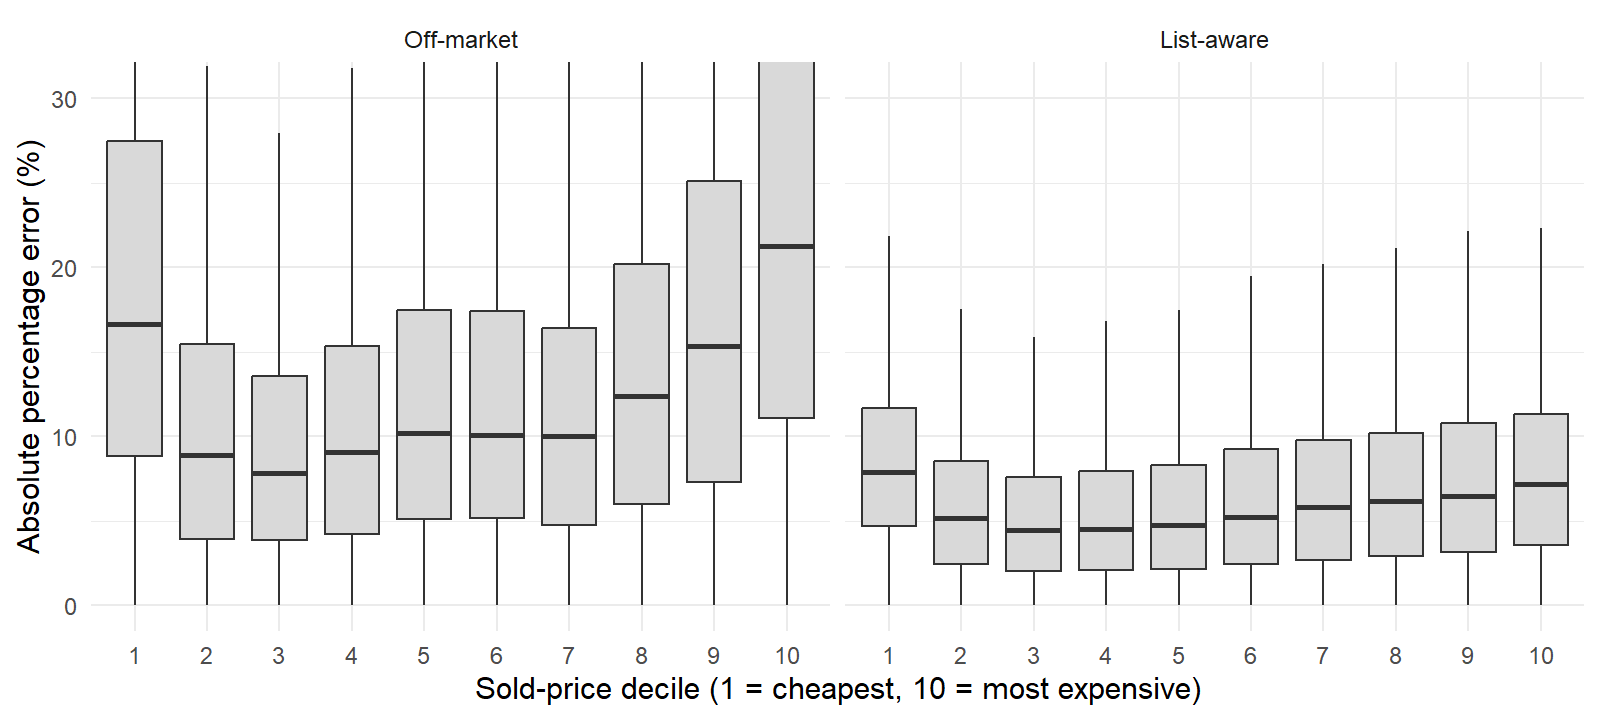
\includegraphics[width=0.72\linewidth]{error_by_price_range.png}}{\todo{figure missing: run the R script}}
\caption{Absolute percentage error by sold-price decile (1 = cheapest, 10 = most expensive). Boxes show the middle 50\%; the vertical axis is cut at the 95th percentile.}
\end{figure}

\textbf{By price.} Off-market errors are smallest in decile \bestDecile{} (MdAPE \bestDecileMd\%) and largest in decile \worstDecile{} (\worstDecileMd\%), which starts at about \$\worstDecilePriceLo. The list-aware model's worst decile is the opposite end, decile \laWorstDecile{} (\laWorstDecileMd\%). A likely reason for the off-market pattern is that expensive homes have fewer comparable sales and a wider spread of prices for similar features, so a model built from attributes alone has less to learn from. For the list-aware model, a fixed dollar gap between list and sold price is a larger percentage on a cheap home.

\textbf{By type, month and place.} The hardest house type is \worstType{} (MdAPE \worstTypeMd\%) and the easiest is \bestType{} (\bestTypeMd\%); Table~\ref{tab:type} in the appendix lists all types. We suspect co-op apartments are hard because their prices depend on maintenance fees and ownership structure, which are not in the data. By month, errors range from \bestMonthMd\% in \bestMonth{} to \worstMonthMd\% in \worstMonth{}, a modest spread; the worst month is the first validation fold, which has the shortest training history. The hardest municipality is \worstMuni{} (\worstMuniMd\%). By community (132 with at least 30 validation homes, from the 100-tree run), the hardest are Hazelfield (25.8\%, 68 homes), Chestnutridge (23.1\%, 32 homes) and Maplepark (21.0\%, 36 homes), and the easiest are Oakcrest (5.1\%) and Pinevale (7.2\%). We have not checked why; a plausible reason is that the hard communities contain more expensive or more varied homes, which would match the price pattern above.


\textbf{What drives predictions.} Permutation importance (Figure~\ref{fig:imp}, appendix) shows the off-market forest relies most on \texttt{\offTopA}, \texttt{\offTopB} and \texttt{\offTopC}; the list-aware forest relies most on \texttt{\laTopA}, \texttt{\laTopB} and \texttt{\laTopC}.


\section{Limitations}
The list-aware model over-predicts by about \laBiasPct\% at the median; a simple correction (for example re-centring the predicted sale-to-list ratio on recent months) is the most promising fix, but we did not have time to build and validate it. The price index is held flat over the June--September test window, so a sharp rise or fall in the market in those months would show up as a bias in every prediction; for the list-aware model we extrapolate it instead, which helped in validation but is a riskier bet over a four-month horizon. Forest settings were fixed, not tuned, and each model uses a single random seed. The remark features come from hand-written keyword lists, which will miss wording we did not anticipate. Location enters as raw categories and coordinates, with no neighbour-based features. With more time we would tune the forest, compare against gradient boosting, add spatial neighbour features, and produce prediction intervals.

\section*{Outside data}
\begin{tabular}{lll}
\toprule
Source & URL & Periods covered \\
\midrule
\textit{None} & & \\
\bottomrule
\end{tabular}

\section*{Reproducing our results}
Install R with the packages \texttt{ranger, dplyr, readr, lubridate, stringr, ggplot2, tidyr} (the script installs missing ones). The script downloads the data from Hugging Face on first run, so it needs an internet connection, and takes roughly 15--40 minutes. \\
\texttt{Rscript ssu\_random\_forest\_v2.R}\\
It writes \texttt{submissions/submission\_off\_market.csv}, \texttt{submissions/submission\_list\_aware.csv}, the report tables in \texttt{reports/}, and the figures in \texttt{figures/}.

\appendix
\section*{Appendix}
\begin{table}[h]
\centering
\IfFileExists{../reports/error_by_type.tex}{\begin{tabular}{lrrr}
\toprule
House type & Homes (off-mkt.) & Off-market MdAPE (\%) & List-aware MdAPE (\%) \\
\midrule
Co-Op Apt & 48 & 14.72 & 4.74 \\
Semi-Detached & 1034 & 13.10 & 6.35 \\
Detached & 3123 & 13.00 & 7.29 \\
Freehold Townhouse & 405 & 12.28 & 6.80 \\
Condo Apt & 4843 & 10.47 & 4.70 \\
Condo Townhouse & 616 & 8.88 & 6.17 \\
\bottomrule
\end{tabular}
}{}
\caption{Median absolute percentage error by house type, validation months.}
\label{tab:type}
\end{table}

\begin{figure}[h]
\centering
\IfFileExists{../figures/importance.png}{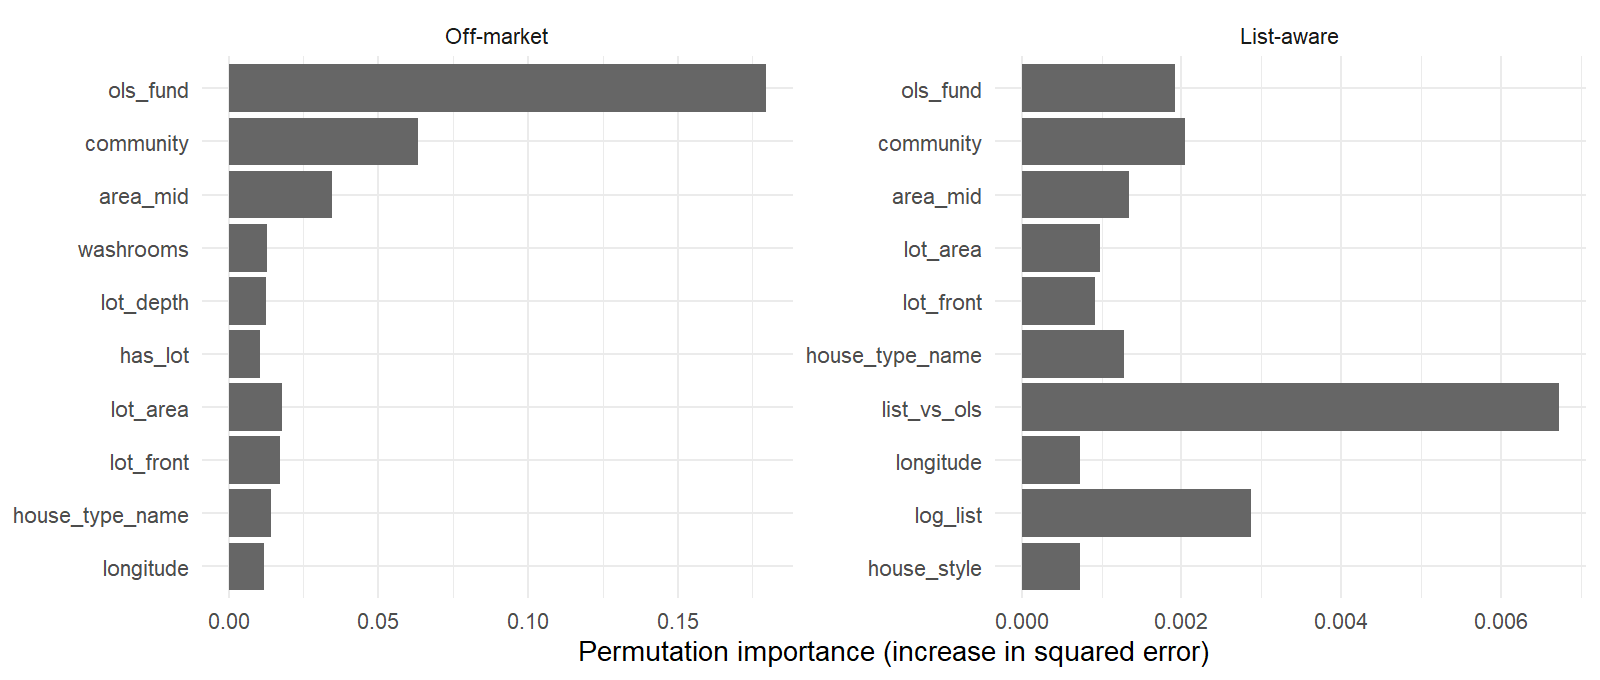
\includegraphics[width=0.8\linewidth]{importance.png}}{\todo{figure missing: run the R script}}
\caption{Top-10 permutation importance in the final forests.}
\label{fig:imp}
\end{figure}

\end{document}
